
\section{Rückblick}

\begin{frame}
  {Erinnerung an letzte Woche: Grammatik}
  \pause
  \begin{itemize}[<+->]
    \item unbewusste Verarbeitung → Akzeptabilität
    \item Gesetzmäßigkeiten = Regularitäten
    \item \alert{System} von Gesetzmäßigkeiten
    \item \alert{definiertes} System → Grammatikalität
    \item \alert{Kern}: Klassen\slash Regularitäten mit hoher Typenfrequenz\\
      Peripherie: niedrige Typenfrequenz
    \item Norm = Beschreibung des Grundkonsenses
  \end{itemize}
\end{frame}

\begin{frame}
  {Erinnerung an letzte Woche: Didaktik}
  \pause
  \begin{itemize}[<+->]
    \item Ziel des Deutschunterrichts: \alert{Bildungssprache}
    \item Bildungssprache + Schriftlichkeit + Norm
    \item Sprachbetrachtung im Alltag
    \item Sprachbetrachtung als Lehrkonzept
    \item Unterricht: \alert{systematisch}, \alert{Form-Funktion}, \alert{induktiv}
    \vspace{\baselineskip}
  \item \rot{Die Grammatik für Studierende des Lehramts ist eine völlig andere\\
      als die, die sie später an Schulkinder und Jugendliche vermitteln!}
  \end{itemize}
\end{frame}

\begin{frame}
  {Der Fragebogen}
  \pause
  \centering
  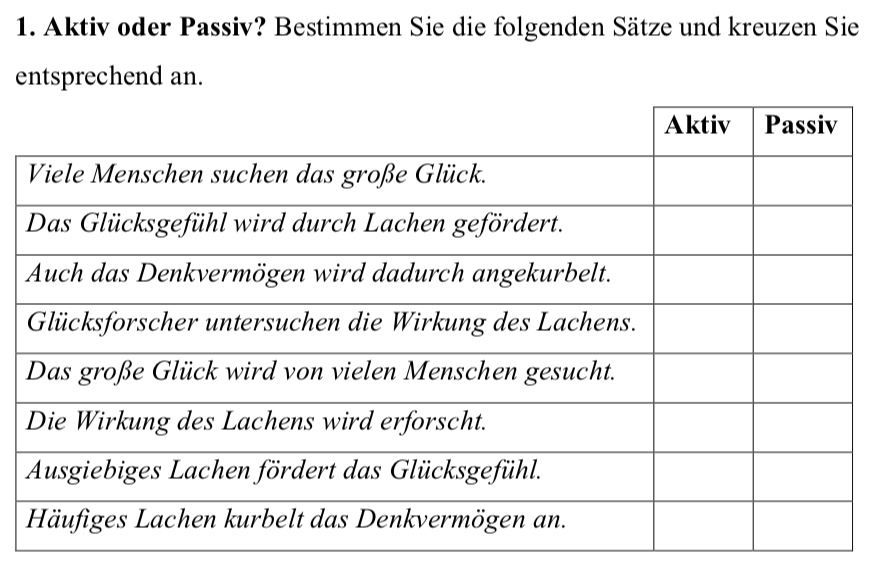
\includegraphics[width=0.75\textwidth]{graphics/01}
\end{frame}

\begin{frame}
  {Der Fragebogen}
  \centering
  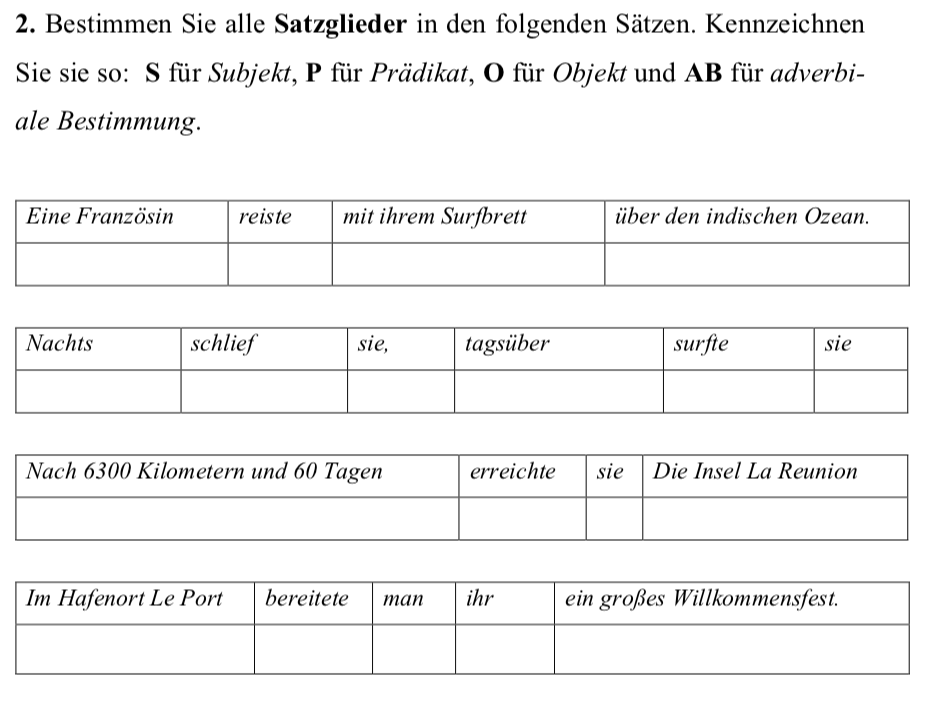
\includegraphics[width=0.75\textwidth]{graphics/02}
\end{frame}

\begin{frame}
  {Der Fragebogen}
  \centering
  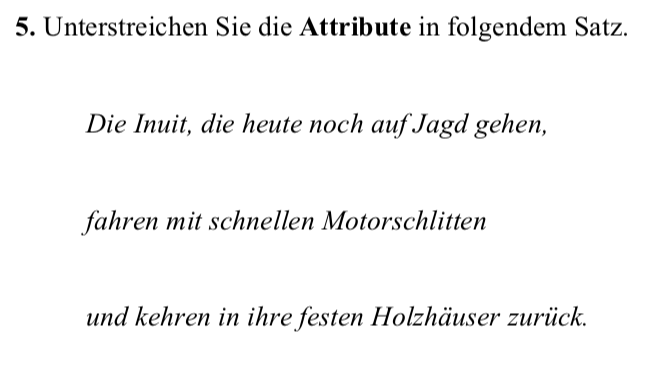
\includegraphics[width=0.75\textwidth]{graphics/03}
\end{frame}

\begin{frame}
  {Der Fragebogen}
  \centering
  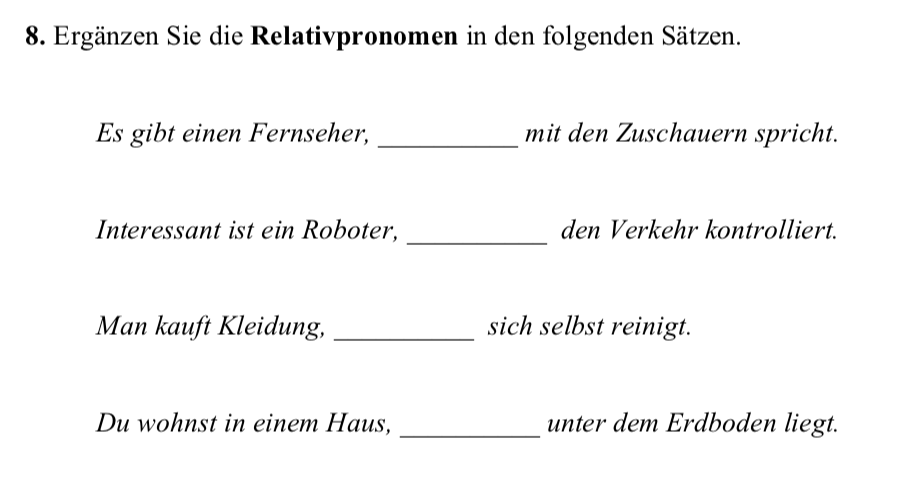
\includegraphics[width=0.75\textwidth]{graphics/04}
\end{frame}

\begin{frame}
  {Auswertung}
  \pause
  \centering
  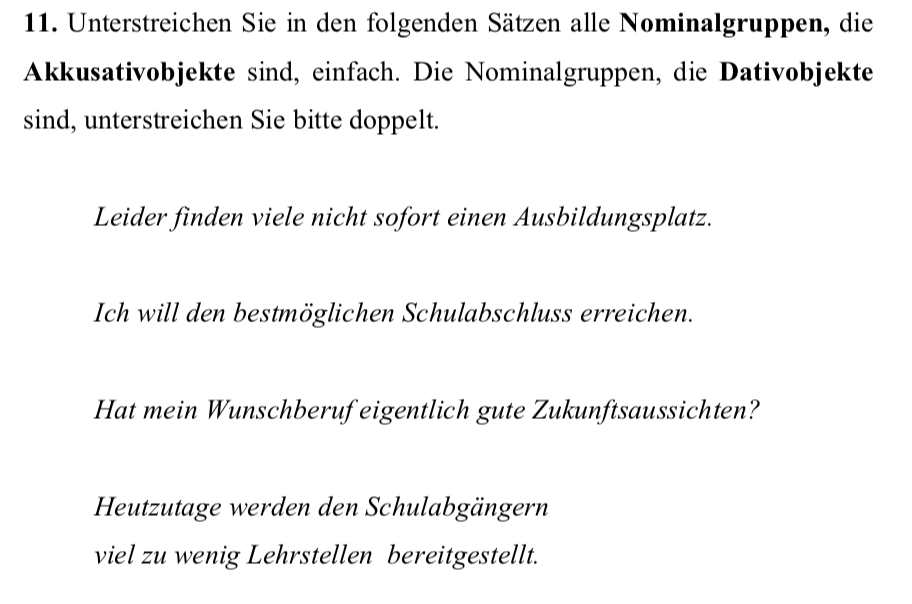
\includegraphics[width=0.75\textwidth]{graphics/05}
\end{frame}

\begin{frame}
  {Auswertung}
  \centering
  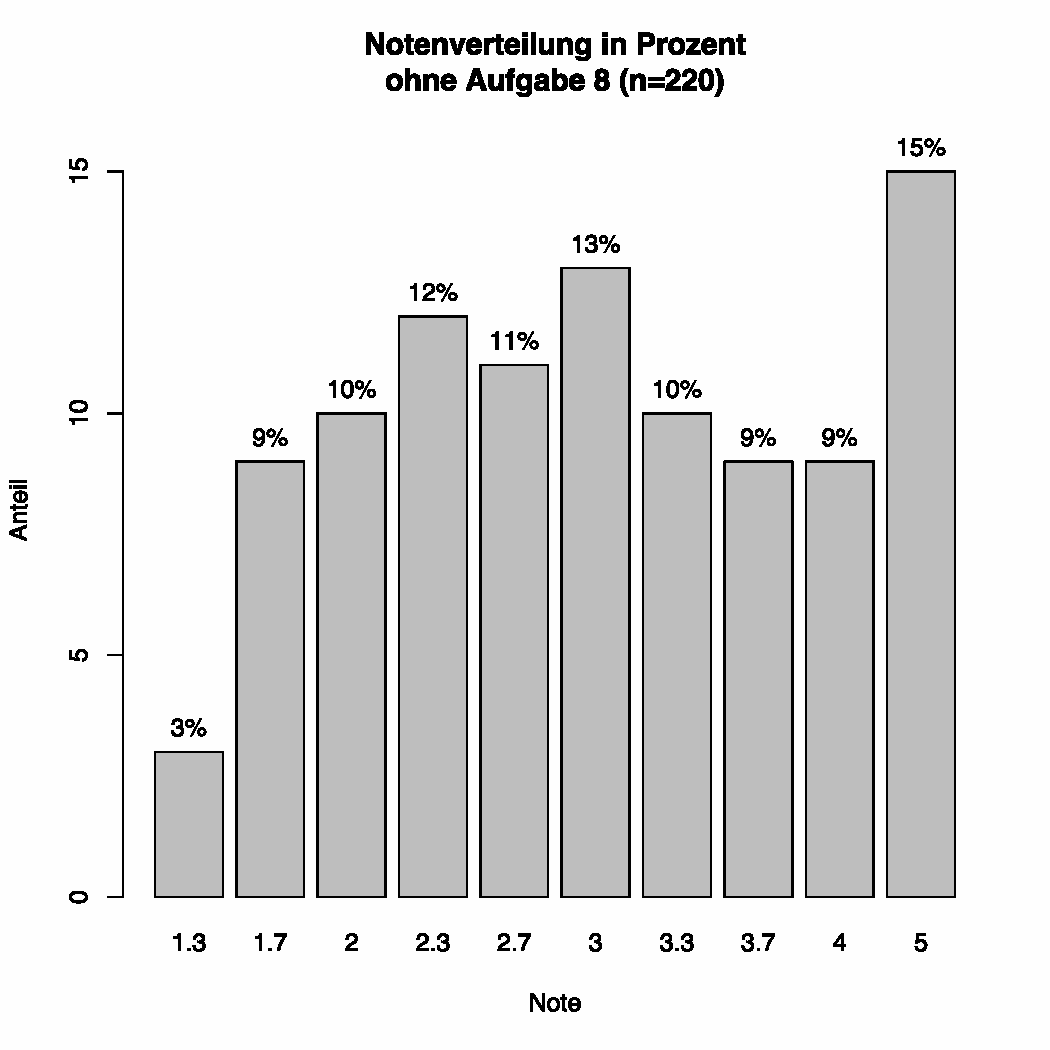
\includegraphics[width=0.6\textwidth]{graphics/notenspiegel}
\end{frame}

\begin{frame}
  {Auswertung}
  \centering
  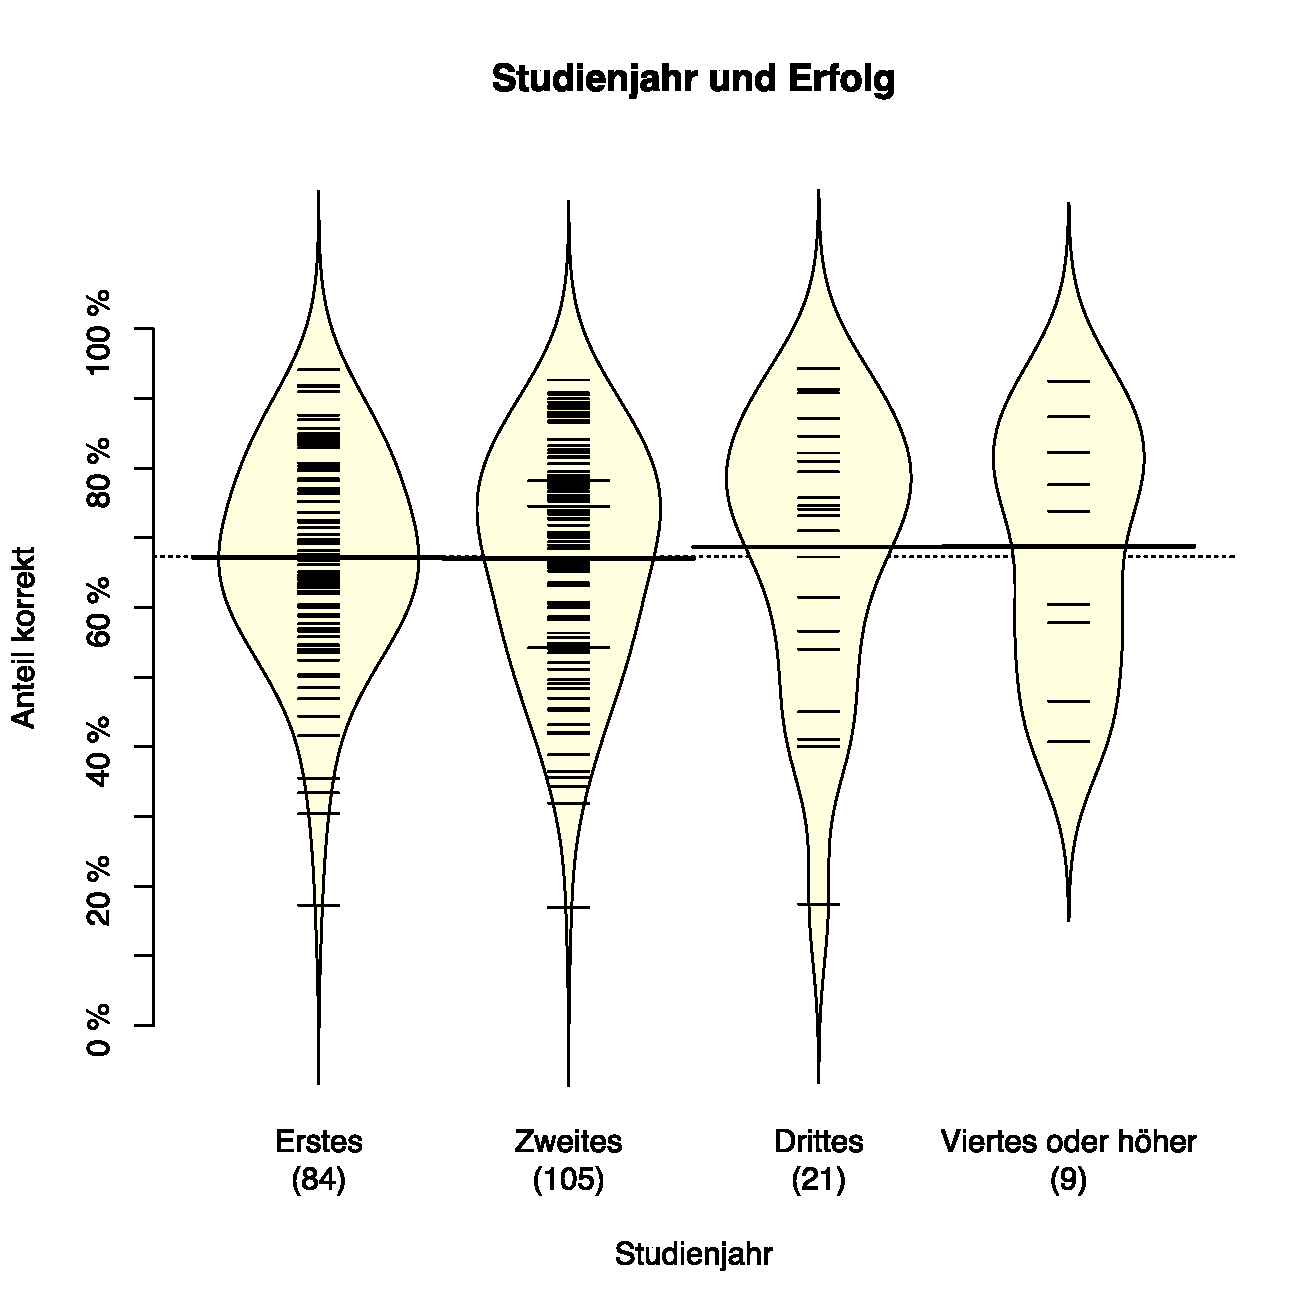
\includegraphics[width=0.6\textwidth]{graphics/semester}
\end{frame}

\begin{frame}
  {Auswertung}
  \centering
  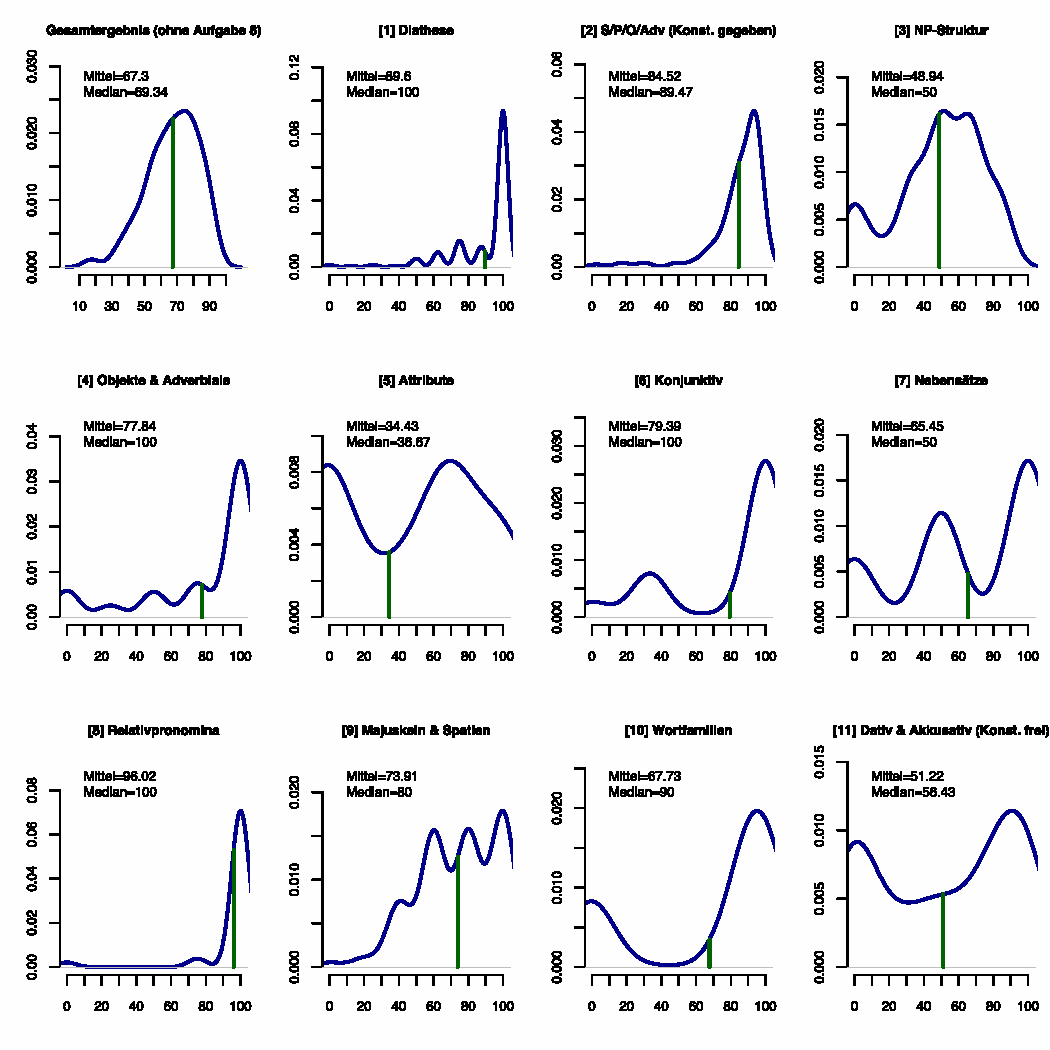
\includegraphics[width=0.6\textwidth]{graphics/prozentverteilung}
\end{frame}

\begin{frame}
  {Wichtige Bücher für das gesamte Studium}
  \pause
  \begin{itemize}[<+->]
    \item Grammatik\slash Linguistik:
      \begin{itemize}[<+->]
        \item \alert{\citet{Eisenberg2013a}}
        \item \alert{\citet{Eisenberg2013b}}
        \item \citet{Mueller2018} (Grammatiktheorie)
      \end{itemize}
    \vspace{\baselineskip}
    \item Linguistisch orientierte Fachdidaktik:
      \begin{itemize}[<+->]
        \item \alert{\citet{Menzel2017}}, dazu \citet{EisenbergMenzel1995}
        \item \alert{\citet{Bredel2013}}
        \item \citet{BredelEa2017} (insbesondere Grundschule)
        \item \citet{BredelPieper2015}
      \end{itemize}
  \end{itemize}
\end{frame}

\section{Phonetik}

\begin{frame}
  {Übersicht}
  \pause
  \begin{itemize}[<+->]
    \item Was ist \alert{Phonetik}?
    \item Was hat Phonetik mit \alert{Bildungssprache} zu tun?
    \item Welche \alert{Organe} sind an der Artikulation beteiligt?
    \item \alert{Wie} werden Vokale und Konsonanten artikuliert?
    \item \alert{Wo} werden Vokale und Konsonanten artikuliert?
    \item Welche Konsonanten und Vokale gibt es im \alert{Standard}?
  \end{itemize}
\end{frame}

\begin{frame}
  {Medien}
  \pause
  \begin{itemize}[<+->]
    \item akustisch
    \item artefaktisch (\zB Schrift)
    \item gestisch
    \vspace{\baselineskip}
  \item Beziehungen?
  \item \textit{Das schreibt man wie man es spricht?}
  \end{itemize}
\end{frame}

\begin{frame}
  {Methode und Ziele}
  \pause
  \begin{itemize}[<+->]
    \item \alert{artikulatorische} Phonetik: Produktion
    \item \alert{perzeptorische} Phonetik: Wahrnehmung
    \item \alert{akustische} Phonetik: physikalische Gestalt
    \vspace{\baselineskip}
  \item Warum \rot{artikulatorisch}?
    \begin{itemize}[<+->]
      \item Transkriptionsalphabete
      \item Grundlage der Phonologie
      \item Grundlage Sprecherziehung i.\,w.\,S.
      \item weitgehend apparatefrei möglich
      \item weitgehend experimentfrei möglich
    \end{itemize}
    \vspace{\baselineskip}
  \item Empfohlene Literatur: \citet{RuesEa2009}
  \end{itemize}
\end{frame}

\begin{frame}
  {Phonetik und Bildungssprache}
  \pause
  \begin{itemize}[<+->]
    \item phonetische Normbeherrschung: Primärmerkmal
    \vspace{0.5\baselineskip}
    \item Prestige
      \begin{itemize}[<+->]
        \item William Labov 1966: (nicht-)rhotische Varietäten des Englischen
        \item drei Kaufhäuser in NYC, drei "`Schichten"'
        \item \textit{r} nach Vokal als \alert{Schichtindikator}
        \item situative Anpassung
      \end{itemize}
  \item Anke Engelkes \textit{Deutschkurs für türkische Mitbürger*innen}
    \vspace{0.5\baselineskip}
    \item \alert{Dialekte, Soziolekte, Kiezsprachen erhalten!}
    \item \rot{Standard lehren!}
    \item zukünftige Lehrpersonen
      \begin{itemize}
        \item Phonetik $\not\subset$ Schulstoff
        \item \rot{Erkennen von Ausspracheproblemen in der Norm}
        \item \alert{richtige Reaktion nur mit phonetischem Wissen}
      \end{itemize}
  \end{itemize}
\end{frame}

\begin{frame}
  {Artikulationsorgane}
  \pause
  \centering
  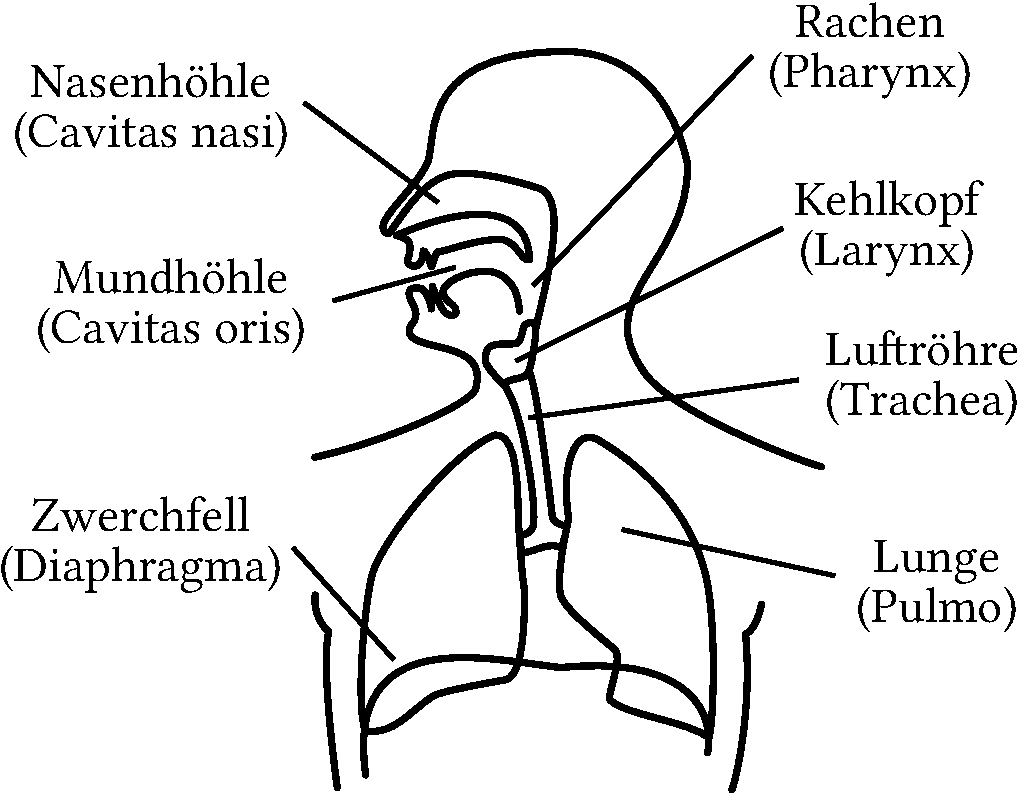
\includegraphics[height=0.7\textheight]{graphics/ueberblick}
\end{frame}

\begin{frame}
  {Mundraum}
  \pause
  \centering
  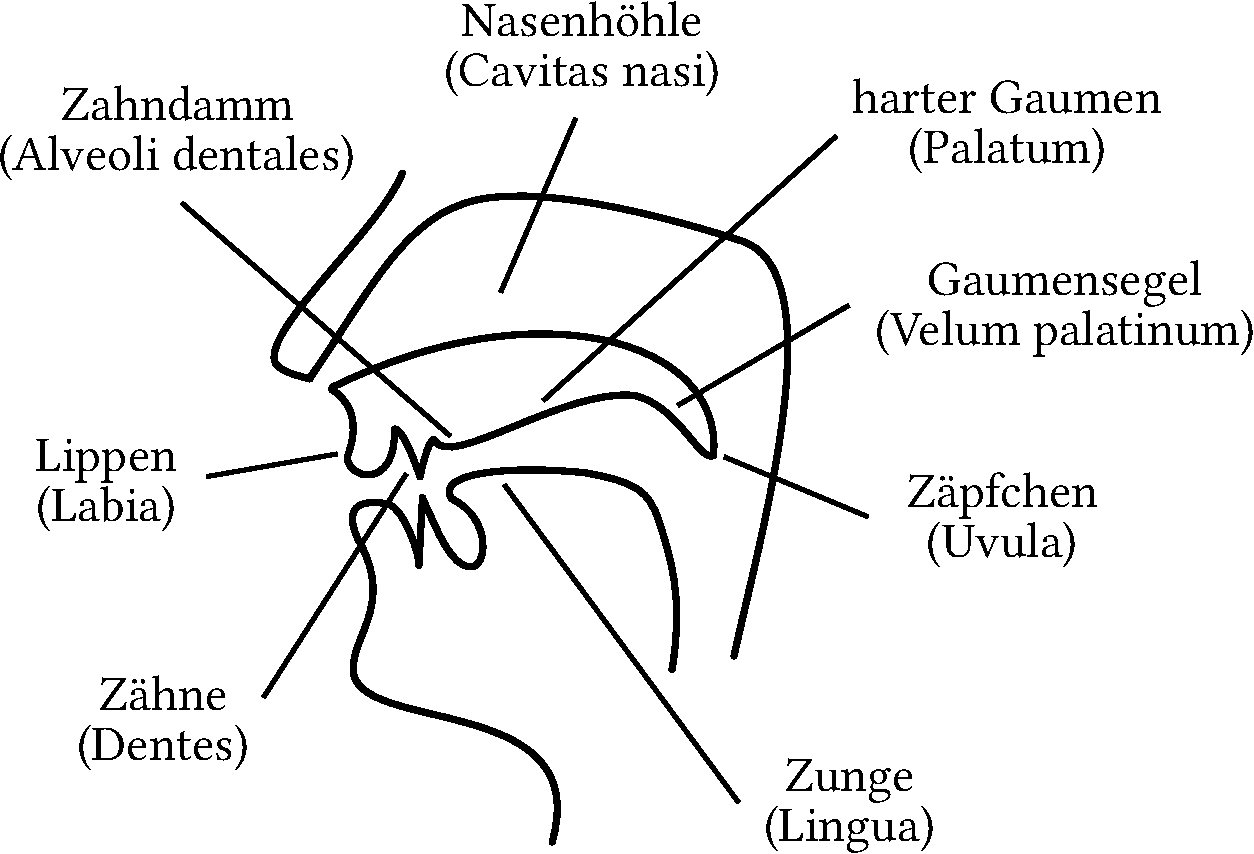
\includegraphics[height=0.7\textheight]{graphics/mundraum}
\end{frame}

\begin{frame}
  {Artikulationen: Konsonanten}
  \pause
    \begin{exe}
      \ex \alert{P}ole, \alert{B}ohle; \alert{T}ank, \alert{D}ank; \alert{g}ilt, \alert{k}illt
      \pause
      \ex \alert{F}ee, \alert{w}eh; hei\alert{ß}er, hei\alert{s}er; schli\alert{ch}, \alert{J}ubel; Ba\alert{ch}, \alert{R}une
      \pause
      \ex \alert{Pf}anne; \alert{Z}irkus; Ma\alert{tsch}
      \pause
      \ex \alert{M}us; \alert{N}uss; Go\alert{ng}
    \end{exe}
    \pause
    \Large
    \begin{itemize}
      \item \alert{Stimmhaftigkeit}
    \end{itemize}
\end{frame}


\begin{frame}
  {Artikulationen: Konsonanten}
  \pause
  \begin{exe}
    \ex \alert{P}a\alert{pp}e, \alert{b}e\alert{b}auen
    \pause
    \ex \alert{T}in\alert{t}e, \alert{d}ul\alert{d}en
    \pause
    \ex \alert{K}na\alert{ck}, \alert{g}e\alert{g}en
    \pause
    \ex Cha\alert{?}ot (Chaos)
    \ex \alert{?}Anfang, \alert{?}über, \alert{?}ohne, \alert{?}Uhr, \dots
  \end{exe}
    \pause
    \Large
    \begin{itemize}
      \item \alert{Plosive}
    \end{itemize}
\end{frame}


\begin{frame}
  {Artikulationen: Konsonanten}
  \pause
  \begin{exe}
    \ex \alert{f}ün\alert{f}, \alert{w}ehe
    \pause
    \ex Bu\alert{s}, \alert{S}ahne
    \pause
    \ex Bä\alert{ch}e, \alert{J}och
    \pause
    \ex Ba\alert{ch}e, \alert{R}asen
  \end{exe}
    \pause
    \Large
    \begin{itemize}
      \item \alert{Frikative}
    \end{itemize}
\end{frame}

\begin{frame}
  {Artikulationen: Konsonanten}
  \pause
  \begin{exe}
    \ex \alert{Pf}anne, To\alert{pf} 
    \pause
    \ex \alert{Z}ange, Schli\alert{tz}
    \pause
    \ex Ma\alert{tsch} (\alert{Ch}ips)
    \pause
    \ex (\alert{Dsch}ungel)
  \end{exe}
    \pause
    \Large
    \begin{itemize}
      \item \alert{Affrikaten}
    \end{itemize}
\end{frame}

\begin{frame}
  {Artikulationen: Konsonanten}
  \pause
  \begin{exe}
    \ex \alert{L}icht, Ba\alert{ll}
  \end{exe}
    \pause
    \Large
    \begin{itemize}
      \item \alert{Approximanten}
    \end{itemize}
    \Zeile
  \pause
  \begin{exe}
    \ex \alert{M}aus, Bau\alert{m}
    \pause
    \ex \alert{N}ase, Ki\alert{nn}
    \pause
    \ex Ri\alert{ng}
  \end{exe}
    \pause
    \Large
    \begin{itemize}
      \item \alert{Nasale}
    \end{itemize}
\end{frame}


\begin{frame}
  {Artikulationen: Vokale}
  \pause
  \begin{exe}
    \ex T\alert{ie}r, T\alert{ü}r; g\alert{u}t
    \pause
    \ex w\alert{e}nig, Fl\alert{ö}te; H\alert{o}se
    \pause
    \ex k\alert{ä}me
    \pause
    \ex B\alert{a}d
    \Zeile
    \pause
    \ex K\alert{i}nd, M\alert{ü}ndel; B\alert{u}s
    \pause
    \ex k\alert{ä}mme, k\alert{ö}nnen; Sch\alert{o}ck
    \pause
    \ex T\alert{a}nne
    \Zeile
    \pause
    \ex s\alert{ei}, Pf\alert{au}, H\alert{eu}
    \Zeile
    \pause
    \ex Tüt\alert{e}, b\alert{e}sonders, Eh\alert{e}, \dots
  \end{exe}
\end{frame}


\begin{frame}
  {Artikulationsarten}
  \pause
  \resizebox{\textwidth}{!}{
  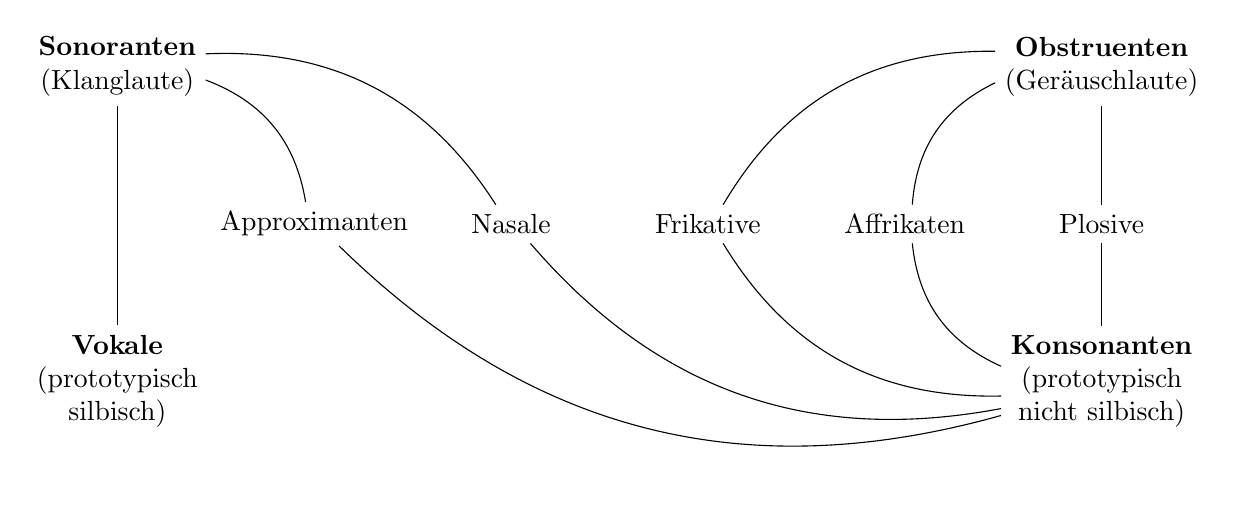
\begin{tikzpicture}[every text node part/.style={align=center}]
    \node (UeVok) at (0,0)  {\textbf{Vokale}\\(prototypisch\\silbisch)};
    \node (UeApr) at (2.5,2)  {Approximanten};
    \node (UeNas) at (5,2)  {Nasale};
    \node (UeFri) at (7.5,2)  {Frikative};
    \node (UeAfr) at (10,2) {Affrikaten};
    \node (UePlo) at (12.5,2)  {Plosive};

    \node (UeSon) at (0,4) {\textbf{Sonoranten}\\(Klanglaute)};
    \node (UeObs) at (12.5,4) {\textbf{Obstruenten}\\(Geräuschlaute)};

    \node (UeKon) at (12.5,0) {\textbf{Konsonanten}\\(prototypisch\\nicht silbisch)};

    \draw (UeSon) to (UeVok);
    \draw [bend left] (UeSon) to (UeApr);
    \draw [bend left] (UeSon) to (UeNas);

    \draw (UeObs) to (UePlo);
    \draw [bend right] (UeObs) to (UeFri);
    \draw [bend right] (UeObs) to (UeAfr);

    \draw [bend right] (UeApr) to (UeKon);
    \draw [bend right] (UeNas) to (UeKon);
    \draw (UePlo) to (UeKon);
    \draw [bend right] (UeFri) to (UeKon);
    \draw [bend right] (UeAfr) to (UeKon);
  \end{tikzpicture}}
\end{frame}

\begin{frame}
  {Artikulationsorte (Konsonanten)}
  \pause
  \begin{exe}
    \ex \alert{P}a\alert{pp}e, \alert{B}irne, \alert{M}ulch
    \pause
    \ex \alert{F}ahne, \alert{W}itz, \alert{Pf}usch
    \pause
    \ex \alert{T}raum, \alert{d}ort, Mi\alert{s}t, \alert{s}ing, \alert{Z}under, \alert{L}uft, \alert{n}och
    \pause
    \ex Bu\alert{sch}, \alert{Tsch}echisch
    \pause
    \ex schle\alert{ch}t, \alert{J}unge
    \pause
    \ex Ro\alert{ck}, \alert{G}abe, Kli\alert{ng}e
    \pause
    \ex wa\alert{ch}, \alert{r}ütteln
    \pause
    \ex \alert{?}offen, \alert{h}och
  \end{exe}
\end{frame}


\begin{frame}
  {Welche Konsonanten gibt es?}
  \centering
  \resizebox{0.7\textwidth}{!}{
  \begin{tabular}{rccccccccc}
    \toprule
    \multicolumn{1}{c}{} & \Sw{\textbf{bilabial}} & \Sw{\textbf{labiodental}} & \Sw{\textbf{alveolar}} & \Sw{\textbf{palatoalveolar}} & \Sw{\textbf{palatal}} & \Sw{\textbf{velar}} & \Sw{\textbf{uvular}} & \Sw{\textbf{laryngal}} \\
    \midrule
    \textbf{stl.\ Plosiv} & p &  & t &  &  & k &  & ʔ \\
    \textbf{sth.\ Plosiv} & b &  & d &  &  & g &  &  \\
    \textbf{stl.\ Frikativ} &  & f & s & ʃ & ç &  & χ & h \\
    \textbf{sth.\ Frikativ} &  & v & z &  & ʝ &  & ʁ &  \\
    \textbf{stl.\ Affrikate} &  & p͡f & t͡s & t͡ʃ &  &  &  &  \\
    \textbf{lateraler Approximant} &  &  & l &  &  &  &  &  \\
    \textbf{Nasal} & m &  & n &  &  & ŋ &  &  \\
    \bottomrule
  \end{tabular}  
  }
\end{frame}


\begin{frame}[fragile]
  {Welche Vokale gibt es?}
  \begin{center}
  \resizebox{0.6\textwidth}{!}{
  \begin{tikzpicture}[scale=2.5,baseline=default]
    \large
    \tikzset{
      vowel/.style={fill=white, anchor=mid, text depth=0ex, text height=1ex},
      dot/.style={circle,fill=black,minimum size=0.4ex,inner sep=0pt,outer sep=-1pt},
    }

    \coordinate (hf) at (0,2); % high front
    \coordinate (hb) at (2,2); % high back
    \coordinate (lf) at (1,0); % low front
    \coordinate (lb) at (2,0); % low back
    \def\V(#1,#2){barycentric cs:hf={(3-#1)*(2-#2)},hb={(3-#1)*#2},lf={#1*(2-#2)},lb={#1*#2}}

    % Chart key (vorne -- hinten).
    \draw [{Latex[round]}-] (\V (-.25,0))   -- (\V (-.25,.5)) node [above left] {\footnotesize vorne};
    \draw [-{Latex[round]}] (\V (-.25,1.5)) -- (\V (-.25,2))  node [above left] {\footnotesize hinten};
    \path (\V (-.25,1)) node[above] {\footnotesize zentral};

    % Chart key (hoch--tief).
    \draw [{Latex[round]}-] (\V (0,-.25)) -- +(270:.5cm)  node [above right,rotate=90] (vokaltrapez1) {\footnotesize hoch};
    \draw [{Latex[round]}-] (\V (3,-2.5)) -- +(270:-.5cm) node [above left,rotate=90] (vokaltrapez2) {\footnotesize tief};
    \path (\V (1.5,-1)) node[above,rotate=90] {\footnotesize mittel};

    % Grid. 
    \draw [gray, thick] (\V(0,0)) -- (\V(0,2));
    \draw [gray, thick] (\V(1,0)) -- (\V(1,2));
    \draw [gray, thick] (\V(2,0)) -- (\V(2,2));
    \draw [gray, thick] (\V(3,0)) -- (\V(3,2));
    \draw [gray, thick] (\V(0,0)) -- (\V(3,0));
    \draw [gray, thick] (\V(0,1)) -- (\V(3,1));
    \draw [gray, thick] (\V(0,2)) -- (\V(3,2));

    % Unrounded-rounded pairs.
    \path (\V(0,0))     node[vowel, left]     {i} node[vowel, right] (y) {y} node[dot] {};
    \path (\V(0.5,0.5)) node[vowel, left]     {ɪ} node[vowel, right] (Y) {ʏ} node[dot] {};
    \path (\V(1,0))     node[vowel, left]     {e} node[vowel, right] (e) {ø} node[dot] {};
    \path (\V(2,0))     node[vowel, left] (E) {ɛ} node[vowel, right] (ee) {œ} node[dot] {};

    % Unpaired symbols.
    \path (\V(1.5,1))    node [vowel] (schwa)  {ə};
    \path (\V(2.5,1))    node [vowel] (schwaa) {ɐ};
    \path (\V(3,1))      node [vowel] (a)      {a};
    \path (\V (2,2))     node [vowel] (oo)     {ɔ};
    \path (\V (1,2))     node [vowel] (o)      {o};
    \path (\V (0,2))     node [vowel] (u)      {u};
    \path (\V (0.5,1.5)) node [vowel] (uu)     {ʊ};

    \path (a)  edge [-{Latex[round]}, bend right=15] (oo);
    \path (a)  edge [-{Latex[round]}, bend left=15]  (E);
    \path (oo) edge [-{Latex[round]}, bend right=15] (ee);
  \end{tikzpicture}
  }
  \end{center}
\end{frame}

\begin{frame}
  {Artikulation anschaulich}
  \vspace{2\baselineskip}
  \centering
  \Large Artikulationsfilme\dots
\end{frame}


\begin{frame}
  {Besonderheiten: Endrand-Desonorisierung}
  \pause
  \begin{exe}
    \ex\label{ex:auslautverhaertung011}
    \begin{xlist}
      \ex{\label{ex:auslautverhaertung012} weck [vɛk]}
      \ex{\label{ex:auslautverhaertung013} Weg [veːk]}
      \ex{\label{ex:auslautverhaertung014} Weges [veːgəs]}
    \end{xlist}
  \pause
    \ex\label{ex:auslautverhaertung015}
    \begin{xlist}
      \ex{\label{ex:auslautverhaertung016} bat [baːt]}
      \ex{\label{ex:auslautverhaertung017} Bad [baːt]}
      \ex{\label{ex:auslautverhaertung018} Bades [baːdəs]}
    \end{xlist}
  \pause
    \ex\label{ex:auslautverhaertung019}
    \begin{xlist}
      \ex{\label{ex:auslautverhaertung020} Flop [flɔp]}
      \ex{\label{ex:auslautverhaertung021} Lob [loːp]}
      \ex{\label{ex:auslautverhaertung022} Lobes [loːbəs]}
    \end{xlist}
  \end{exe}
\end{frame}


\begin{frame}
  {Besonderheiten: Silbische Nasale und Liquiden}
  \pause
  \begin{exe}
    \ex\label{ex:silbischenasaleundapproximanten023}
    \begin{xlist}
      \ex{laufen [la͡ɔfn̩]~\slash~[la͡ɔfən]}
      \ex{haben [habm̩]~\slash~[habən]}
      \ex{kriegen [kʁiːgŋ̩]~\slash~[kʁiːgən]}
      \ex{rotem [ʁoːtm̩]~\slash~[ʁoːtəm]}
      \ex{Bündel [bʏndl̩]~\slash~[bʏndəl]}
    \end{xlist}
  \end{exe}
\end{frame}

\begin{frame}
  {Besonderheiten: \textit{r}-Laute}
  \pause
  \begin{exe}
    \ex\label{ex:orthographischesr030}
    \begin{xlist}
      \ex{Tier [ti͡ɐ], Tür [ty͡ɐ]}
      \ex{Kirche [kɪ͡əçə], Bürde [bʏ͡ədə]}
      \ex{nur [nu͡ɐ]}
      \ex{Bursche [bʊ͡əʃə]}
      \ex{der [de͡ɐ], Stör [ʃtø͡ɐ]}
      \ex{Chor [ko͡ɐ]}
      \ex{gern [gɛ͡ən], Börse [bœ͡əzə]}
      \ex{Korn [kɔ͡ən]}
      \ex{Bar [ba͡ə]}
      \ex{knarr [kna͡ə]}
    \end{xlist}
  \end{exe}
\end{frame}


\begin{frame}[fragile]
  {Sekundäre Vokale}
  \begin{center}
  \resizebox{0.6\textwidth}{!}{
  \begin{tikzpicture}[scale=3,baseline=default]
    \large
    \tikzset{
    vowel/.style={fill=white, anchor=mid, text depth=0ex, text height=1ex},
    dot/.style={circle,fill=black,minimum size=0.4ex,inner sep=0pt,outer sep=-1pt},
    }

    \coordinate (hf) at (0,2); % high front
    \coordinate (hb) at (2,2); % high back
    \coordinate (lf) at (1,0); % low front
    \coordinate (lb) at (2,0); % low back
    \def\V(#1,#2){barycentric cs:hf={(3-#1)*(2-#2)},hb={(3-#1)*#2},lf={#1*(2-#2)},lb={#1*#2}}

    % Chart key (vorne -- hinten).
    \draw [{Latex[round]}-] (\V (-.25,0)) -- (\V (-.25,.5))  node [above left] {\footnotesize vorne};
    \draw [-{Latex[round]}] (\V (-.25,1.5)) -- (\V (-.25,2)) node [above left] {\footnotesize hinten};
    \path (\V (-.25,1)) node[above] {\footnotesize zentral};

    % Chart key (hoch--tief).
    \draw [{Latex[round]}-] (\V (0,-.25)) -- +(270:.5cm)  node [above right,rotate=90] (vokaltrapez1) {\footnotesize hoch};
    \draw [{Latex[round]}-] (\V (3,-2.5)) -- +(270:-.5cm) node [above left,rotate=90] (vokaltrapez2) {\footnotesize tief};
    \path (\V (1.5,-1)) node[above,rotate=90] {\footnotesize mittel};

    % Grid.
    \draw [gray, thick] (\V(0,0)) -- (\V(0,2));
    \draw [gray, thick] (\V(1,0)) -- (\V(1,2));
    \draw [gray, thick] (\V(2,0)) -- (\V(2,2));
    \draw [gray, thick] (\V(3,0)) -- (\V(3,2));
    \draw [gray, thick] (\V(0,0)) -- (\V(3,0));
    \draw [gray, thick] (\V(0,1)) -- (\V(3,1));
    \draw [gray, thick] (\V(0,2)) -- (\V(3,2));

    % Unrounded-rounded pairs.
    \path (\V(0,0))     node[vowel, left] {i} node [vowel, right] (y)  {y} node [dot] {};
    \path (\V(0.5,0.5)) node[vowel, left] {ɪ} node [vowel, right] (Y)  {ʏ} node [dot] {};
    \path (\V(1,0))     node[vowel, left] {e} node [vowel, right] (e)  {ø} node [dot] {};
    \path (\V(2,0))     node[vowel, left] {ɛ} node [vowel, right] (ee) {œ} node [dot] {};

    % Unpaired symbols.
    \path (\V(1.5,1))    node [vowel] (schwa)  {ə};
    \path (\V(2.5,1))    node [vowel] (schwaa) {ɐ};
    \path (\V(3,1))      node [vowel] (a)      {a};
    \path (\V (2,2))     node [vowel] (oo)     {ɔ};
    \path (\V (1,2))     node [vowel] (o)      {o};
    \path (\V (0,2))     node [vowel] (u)      {u};
    \path (\V (0.5,1.5)) node [vowel] (uu)     {ʊ};

    % Connections.
    \path (y) edge  [-{Latex[round]}, bend right=3]  (schwaa);
    \path (e) edge  [-{Latex[round]}, bend right=10] (schwaa);
    \path (ee) edge [-{Latex[round]}, bend left=20]  (schwa);
    \path (a) edge  [-{Latex[round]}, bend right=40] (schwa);
    \path (oo) edge [-{Latex[round]}, bend right=20] (schwa);
    \path (o) edge  [-{Latex[round]}, bend left=15]  (schwaa);
    \path (u) edge  [-{Latex[round]}, bend left=10]  (schwaa);
    
    \draw [-{Latex[round]}]             (Y)  -- (schwa);
    \draw [-{Latex[round]}, bend right] (uu) -- (schwa);
  \end{tikzpicture}
  }
  \end{center}
\end{frame}


\section{Vorschau}

\begin{frame}
  {Von der Phonetik zur Phonologie}
  \pause
  \begin{itemize}[<+->]
    \item Wiederholung\slash Übung der Phonetik
    \item Vorkommen von Segmenten: nicht alle überall
    \item System: zugrundeliegende Segmente und Prozesse
    \item Vorgriff auf die Graphematik: Buchstaben und Segmente
      \Zeile
    \item \rot{Lesen Sie bitte: Kapitel 5, S.~111--123}
    \item \alert{Wiederholen: Kapitel 4, S.~104--108}
  \end{itemize}

  \pause
  \pause
  \pause
  \pause
  \pause
\end{frame}


